\section{Method}
\label{sec:method}

Figure~\ref{fig:overview} shows the model. An always-on path turns every 40\,ms chunk of audio into cheap features for 64 frequency regions. A selective path keeps an expensive persistent state for each region and updates only a budget-limited subset of regions per chunk. A controller decides which subset to update, and a readout combines both paths into frame-level predictions. The selection method, i.e., the skip-harm target, the controller and the budget-exact selection rule, does not depend on the recurrent cell or on the graph topology: it only needs a cell that can update a subset of nodes and a readout whose output can be compared. We describe it with an AGN-Net-style cell, which carries over AGN-Net's localized updates, and evaluate it with two cells, two graph topologies and two datasets (Section~\ref{sec:experiments}).

\begin{figure}[H]
\begin{adjustwidth}{-\extralength}{0cm}
\centering
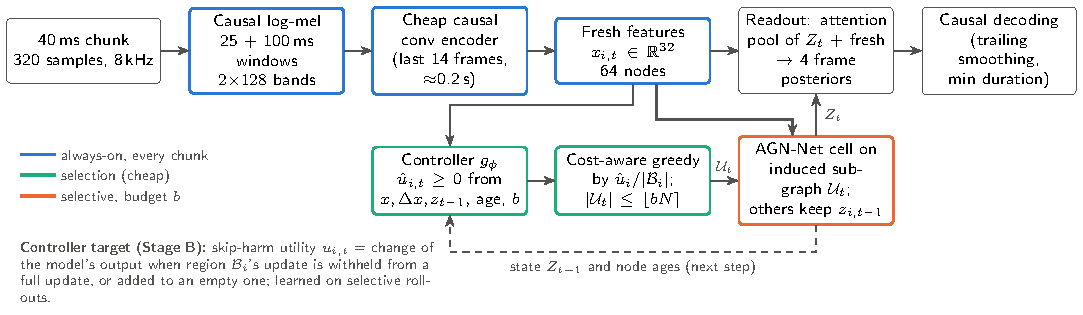
\includegraphics[width=\linewidth]{figures/overview.pdf}
\end{adjustwidth}
\caption{Overview of Event-Aware AGN-Net. Each 40\,ms chunk is processed by a causal two-resolution log-mel front end and a cheap convolutional encoder, giving fresh features $x_{i,t}$ for $N{=}64$ frequency-region nodes. A controller scores each seed region $\B_i$, and a cost-aware greedy picks an update set $\U_t$ whose size never exceeds $\lfloor bN\rceil$. The AGN-Net cell updates only the nodes in $\U_t$, on the subgraph induced by $\U_t$; all other nodes keep their state. The readout combines the pooled graph state with the fresh features. The controller is trained to predict the \emph{skip-harm utility}, i.e., how much the output changes when a region's update is withheld.}
\label{fig:overview}
\end{figure}

\subsection{Problem Formulation}
Audio arrives in 40\,ms chunks. After chunk $t$, the model must output class posteriors for the four 10\,ms frames in that chunk, using only audio received so far. There are $C{=}8$ classes: background plus the seven SPRSound event types (Normal, Rhonchi, Wheeze, Stridor, Coarse Crackle, Fine Crackle, Wheeze+Crackle). Events are decoded from the frame posteriors. The model keeps a state $z_{i,t}$ for each of $N$ graph nodes. A budget $b\in(0,1]$ limits how many node states may be recomputed per chunk. The goal is to choose, at each step, the update set $\U_t$ with $|\U_t|\le\lfloor bN\rceil$ that keeps the output as close as possible to the output of updating every node ($\lfloor\cdot\rceil$ denotes rounding to the nearest integer).

\subsection{Always-On Encoder}
Audio is processed at its native 8\,kHz. For each 10\,ms frame we compute two log-mel spectra (128 bands, 50--4000\,Hz) with 25\,ms and 100\,ms Hann windows that end at the current frame, so no future samples are used. Features are standardized with fixed statistics from the training set. A causal $5{\times}3$ convolution (2$\to$16 channels) runs at the frame rate, the four frames of a chunk are averaged, and a second causal $5{\times}3$ convolution (16$\to$32 channels, frequency stride 2) runs at the chunk rate, followed by LayerNorm. This gives a 32-dimensional feature $x_{i,t}$ for each of the 64 frequency regions. The encoder only sees the last 14 frames (about 0.2\,s), so longer temporal context must come from the graph state.

\subsection{Persistent Acoustic Graph}
\label{sec:graph}
Each node $i$ is anchored to a fixed pair of adjacent mel channels at both resolutions, so its identity is stable over time while its features change. Edges connect nodes at frequency distance 1 and 2. This chain is the simplest topology, and it cannot pass evidence between distant harmonics in one step. Wheezes and stridor are (quasi-)harmonic, with energy at integer multiples of a fundamental frequency, so we also build a \emph{harmonic graph} that additionally links each node to the nodes nearest to twice and three times its centre frequency (relative mismatch below 6\%). This adds 82 edges, with at most 8 neighbours per node. Selection, budgets and training are unchanged; only the regions $\B_i$ become larger. Each node keeps a 96-dimensional state. For nodes in the update set $\U_t$, the AGN-Net cell computes
\begin{align}
h^{(0)}_i &= \mathrm{GELU}\big(W_{\mathrm{in}}[x_{i,t};z_{i,t-1}] + e_i\big),\label{eq:cell-first}\\
h^{(\ell)}_i &= \mathrm{ELU}\Big(\sum_{j\in\mathcal{N}_{\U}(i)}\alpha^{(\ell)}_{ij}W^{(\ell)}h^{(\ell-1)}_j+\beta_\ell h^{(\ell-1)}_i\Big),\\
f_i &= \mathrm{LN}\Big(\textstyle\sum_{\ell=0}^{2}\mathrm{softmax}(w)_\ell\,h^{(\ell)}_i\Big),\\
c_i &= \tanh(\mathrm{MLP}(f_i)),\\
\lambda_i &= \sigma\big(w_g^\top[f_i;z_{i,t-1}]+b_g\big),\\
z_{i,t} &= (1-\lambda_i)\,z_{i,t-1}+\lambda_i\,c_i,\label{eq:cell-update}
\end{align}
for layers $\ell=1,2$. Nodes outside $\U_t$ keep their state, $z_{i,t}=z_{i,t-1}$. Here GELU and ELU are the Gaussian-error and exponential linear units, LN is layer normalization, MLP is a multilayer perceptron, $e_i$ is a learned node embedding, $\alpha^{(\ell)}_{ij}$ are graph-attention weights~\cite{velickovic2018graph} computed only over neighbours inside $\U_t$ (AGN-Net's induced-subgraph update~\cite{islam2026agnnet}), $\beta_\ell$ are learned residual weights, and $w$ fuses the layers. AGN-Net's temporal-momentum update is kept, with its global momentum replaced by a per-node gate $\lambda_i$. When $\U_t$ contains all nodes, we call the model the \emph{full-update} model. For the plain graph-GRU cell used in Section~\ref{sec:generality}, $z_{i,t}=\mathrm{GRU}\big(\mathrm{GELU}(W[x_{i,t};\bar z_{\mathcal{N}(i),t-1}]+e_i),\,z_{i,t-1}\big)$ with $\bar z_{\mathcal{N}(i)}$ the mean of the neighbour states; a selective update applies this only to $i\in\U_t$ and reads the (possibly stale) states of all neighbours, so for this cell the boundary defect of Proposition~\ref{prop:bound} is zero.

The readout pools the node states with attention, $g_t=\sum_i\mathrm{softmax}_i(w_s^\top z_{i,t})\,z_{i,t}$, concatenates the mean and maximum of the fresh features over nodes, and maps the result through a two-layer MLP to four frame posteriors. The fresh-feature input lets the readout react to the current chunk even when few states were updated. The full model has about 108,000 parameters.

\subsection{Budgeted Region Selection}
\label{sec:selection}
Selecting a seed node $i$ updates its region $\B_i=\{i\}\cup\mathcal{N}(i)$ of 3--5 nodes (up to 9 on the harmonic graph), so the actual update set is the union of the selected regions. We therefore count the budget in updated nodes, $|\U_t|\le\lfloor bN\rceil$, not in seeds. Each policy gives every region a non-negative score $s_{i,t}$ (a region total). A greedy rule visits the regions in decreasing order of the per-node score $s_{i,t}/|\B_i|$, and adds a region if it brings at least one new node and still fits the budget. This is a heuristic for a budgeted coverage problem~\cite{khuller1999budgeted}. We use the per-node score, rather than the usual score per newly covered node, because the latter makes regions overlapping an already chosen region look almost free, and the update set then grows as one contiguous block regardless of score.

To avoid states becoming arbitrarily stale, nodes whose state is at least $A$ steps old are refreshed first. These refreshes count against the same budget. As a result, every policy performs exactly the same number of node updates per step. Refreshing all $N$ nodes once every $A$ steps costs at most $N/A$ updates per step, i.e., a share $1/(Ab)$ of the budget, so a fixed threshold weighs most on the smallest budgets. The main experiments use a fixed $A{=}50$ steps (2\,s). On long streams (Section~\ref{sec:long}) we also test a budget-adaptive threshold $A(b)=\lceil 12.5/b\rceil$ steps (100, 50 and 25 steps at 12.5\%, 25\% and 50\%), which caps the refresh share at 8\% of the budget.

\subsection{Skip-Harm Utility}
\label{sec:utility}
The controller should prefer regions whose update matters for the output. We measure this directly with one-step counterfactuals. Let $p(Z)$ be the readout's frame posteriors for state $Z$, and $p^{\mathrm{full}}$ and $p^{\mathrm{none}}$ the posteriors if all or no nodes are updated at this step. For region $i$, let $p^{\mathrm{hold}(i)}$ be the posteriors when every node except $\B_i$ is updated, and $p^{\mathrm{only}(i)}$ when only $\B_i$ is updated. With $D$ the Kullback--Leibler (KL) divergence averaged over the four frames, we define
\begin{align}
\Delta^{\mathrm{hold}}_{i,t} &= D\big(p^{\mathrm{full}}\,\|\,p^{\mathrm{hold}(i)}\big),\nonumber\\
\Delta^{\mathrm{add}}_{i,t} &= \big(D(p^{\mathrm{full}}\|p^{\mathrm{none}})-D(p^{\mathrm{full}}\|p^{\mathrm{only}(i)})\big)_+,\nonumber\\
L^{\mathrm{hold}}_{i,t} &= \big(\mathrm{CE}(y,p^{\mathrm{hold}(i)})-\mathrm{CE}(y,p^{\mathrm{full}})\big)_+,\nonumber\\
L^{\mathrm{add}}_{i,t} &= \big(\mathrm{CE}(y,p^{\mathrm{none}})-\mathrm{CE}(y,p^{\mathrm{only}(i)})\big)_+,\nonumber\\
u_{i,t} &= \tfrac12\big(\Delta^{\mathrm{hold}}_{i,t}+\Delta^{\mathrm{add}}_{i,t}\big)+\tfrac{\mu}{2}\big(L^{\mathrm{hold}}_{i,t}+L^{\mathrm{add}}_{i,t}\big),
\label{eq:utility}
\end{align}
where $\mathrm{CE}$ is the frame cross-entropy on labelled frames and $\mu{=}1$. The $\Delta$ terms measure how much the prediction depends on region $i$ when it is removed from a full update and when it is added to an empty one. This two-point estimate is similar in spirit to a Shapley value~\cite{lundberg2017unified}. The $L$ terms add the increase in supervised loss. Computing the targets is cheap: one cell evaluation plus 128 readout evaluations per step for all 64 regions, run on the graphics processing unit (GPU) without gradients. For speed, the intervened regions reuse the state computed with their full neighbourhood.

The targets are one-step proxies. A skipped state stays stale, so a skip can also change later outputs, and repeated skips of the same region compound. Exact multi-step targets would require rolling out every region's counterfactual over the horizon, which multiplies the cost of target generation by the horizon length and makes the target depend on future selections. We therefore keep the one-step target and test directly, in Section~\ref{sec:multistep}, how well it ranks regions by their measured harm over horizons of up to 1\,s and under repeated skips.

\paragraph*{Controller}
The controller uses only information available at inference time: $r_{i,t}=[x_{i,t};\,x_{i,t}-x_{i,t-1};\,z_{i,t-1};\,a_{i,t};\,b]$, where $a_{i,t}$ is the (log-scaled) age of node $i$'s state. A shared per-node layer (24 units) is followed by a 5-tap convolution over neighbouring nodes and a softplus output $\hat u_{i,t}\ge0$, for about 6800 parameters in total. It is trained with a Huber loss between $\log(1+\hat u_{i,t})$ and $\log(1+u_{i,t}/\kappa)$, where $\kappa$ is a fixed target scale ($\kappa{=}0.01$; $0.1$ for the change head below). With the same architecture, inputs and training data we also train three alternative heads: a \emph{change} head that predicts the representation change $\|z^{\mathrm{full}}_{j,t}-z_{j,t-1}\|$ averaged over the region (AGN-Net's objective), a \emph{hold-only} head ($\Delta^{\mathrm{hold}}+\mu L^{\mathrm{hold}}$), and a \emph{label-free} head ($\mu{=}0$).

\subsection{Training}
\label{sec:training}
Training has three stages. \emph{Stage A} trains the encoder, cell and readout with full updates for 40 epochs, using AdamW (peak learning rate $2{\times}10^{-3}$, one-cycle schedule), batches of 32 random 8\,s crops, class-weighted frame cross-entropy, random gain, and frequency masking~\cite{park2019specaugment}. \emph{Stage B} freezes the model and trains the controller heads for 6 epochs on \emph{selective rollouts}. Each batch runs either random selection or one of the learned heads under a random budget, so the controllers see the stale states they will meet at inference time~\cite{ross2011reduction}. \emph{Stage C} fine-tunes the model for 8 epochs under a random policy and budget per batch, with a distillation loss~\cite{hinton2015distilling} towards the stage-A full-update model. The controllers are then refreshed for 2 epochs on the fine-tuned model (stage B$'$). Because one fine-tuned model serves all policies, every policy is evaluated on the same weights. Gradient clipping and a guard that skips non-finite updates keep training stable.

\subsection{Error Analysis}
\label{sec:theory}
Selective updating differs from full updating in two ways: nodes outside $\U_t$ keep stale states (\emph{skip defect}), and nodes inside $\U_t$ miss messages from neighbours outside it (\emph{boundary defect}). AGN-Net~\cite{islam2026agnnet} bounded the first; we add the second. Let $V=\{1,\dots,N\}$ and equip the state space with the norm $\|Z\|_{\infty,2}=\max_{i\in V}\|z_i\|_2$. For the current input $x_t$, let $\Phi_t(Z)=\Phi(Z,x_t)$ denote the full-graph transition, i.e., Equations~(\ref{eq:cell-first})--(\ref{eq:cell-update}) applied to every node on the full graph. For $U\subseteq V$, let $\Phi_t^{U}$ denote the selective transition, which applies Equations~(\ref{eq:cell-first})--(\ref{eq:cell-update}) on the subgraph induced by $U$ to the nodes in $U$ and leaves the other states unchanged, $[\Phi_t^{U}(Z)]_i=z_i$ for $i\notin U$. Both models share weights and inputs and follow
\[
Z^{\mathrm{full}}_t=\Phi_t(Z^{\mathrm{full}}_{t-1}),\qquad Z^{\mathrm{sel}}_t=\Phi_t^{\U_t}(Z^{\mathrm{sel}}_{t-1}),\qquad Z^{\mathrm{full}}_0=Z^{\mathrm{sel}}_0,
\]
and we write $e_t=\|Z^{\mathrm{full}}_t-Z^{\mathrm{sel}}_t\|_{\infty,2}$.

\begin{Proposition}
\label{prop:bound}
Assume that, for each $t$, $\Phi_t$ is $\gamma_t$-Lipschitz in $\|\cdot\|_{\infty,2}$ on a domain that contains the states of both trajectories, with $\gamma_t\ge0$. Define the skip and boundary defects, both evaluated at the selective model's previous state,
\[
\delta^{\mathrm{skip}}_t=\max_{i\notin\U_t}\big\|\Phi_{t,i}(Z^{\mathrm{sel}}_{t-1})-z^{\mathrm{sel}}_{i,t-1}\big\|_2,\qquad
\delta^{\mathrm{bnd}}_t=\max_{i\in\U_t}\big\|\Phi_{t,i}(Z^{\mathrm{sel}}_{t-1})-\Phi^{\U_t}_{t,i}(Z^{\mathrm{sel}}_{t-1})\big\|_2,
\]
where a maximum over an empty node set is zero, and let $d_t=\max\{\delta^{\mathrm{skip}}_t,\delta^{\mathrm{bnd}}_t\}$. Then $e_t\le\gamma_t e_{t-1}+d_t$, and consequently
\[
e_t\le\sum_{s=1}^{t}\Big(\prod_{r=s+1}^{t}\gamma_r\Big)\,d_s ,
\]
where an empty product equals one. If, in addition, $\gamma_t\le\gamma<1$ and $d_t\le\bar\delta$ for all $t$, then $e_t\le\bar\delta(1-\gamma^t)/(1-\gamma)$.
\end{Proposition}
\begin{proof}
Add and subtract $\Phi_t(Z^{\mathrm{sel}}_{t-1})$. By the triangle inequality,
\[
e_t\le\big\|\Phi_t(Z^{\mathrm{full}}_{t-1})-\Phi_t(Z^{\mathrm{sel}}_{t-1})\big\|_{\infty,2}+\big\|\Phi_t(Z^{\mathrm{sel}}_{t-1})-\Phi_t^{\U_t}(Z^{\mathrm{sel}}_{t-1})\big\|_{\infty,2}.
\]
The Lipschitz assumption bounds the first term by $\gamma_t e_{t-1}$. In the second term, skipped nodes keep their previous states, so the maximum row norm over $V\setminus\U_t$ is $\delta^{\mathrm{skip}}_t$, and the maximum row norm over $\U_t$ is $\delta^{\mathrm{bnd}}_t$. The two row sets are disjoint and cover $V$, so the second term equals $d_t$. Hence $e_t\le\gamma_t e_{t-1}+d_t$. Iterating gives $e_t\le(\prod_{r=1}^{t}\gamma_r)\,e_0+\sum_{s=1}^{t}(\prod_{r=s+1}^{t}\gamma_r)\,d_s$, and $e_0=0$. Under $\gamma_t\le\gamma<1$ and $d_t\le\bar\delta$, the sum is at most $\bar\delta\sum_{k=0}^{t-1}\gamma^k=\bar\delta(1-\gamma^t)/(1-\gamma)$.
\end{proof}

For the gated AGN-Net cell, Equation~(\ref{eq:cell-update}) gives an equivalent form of the skip defect: $\Phi_{t,i}(Z^{\mathrm{sel}}_{t-1})-z^{\mathrm{sel}}_{i,t-1}=\lambda^{F}_{i,t}\,(c^{F}_{i,t}-z^{\mathrm{sel}}_{i,t-1})$, so $\delta^{\mathrm{skip}}_t=\max_{i\notin\U_t}\lambda^{F}_{i,t}\|c^{F}_{i,t}-z^{\mathrm{sel}}_{i,t-1}\|_2$, where the gate $\lambda^{F}_{i,t}\ge0$ and the candidate $c^{F}_{i,t}$ are computed on the \emph{full} graph from $Z^{\mathrm{sel}}_{t-1}$, a hypothetical update that the selective model does not perform. Defined through $\Phi_t$, the proposition applies unchanged to the graph-GRU cell, whose boundary defect is zero (Section~\ref{sec:graph}). The argument is a standard perturbation analysis, in which a one-step Lipschitz bound is iterated into a geometric series, as for the hidden states of simple recurrent networks~\cite{mitarchuk2024length}; the application-specific part is the decomposition into skipped-update and induced-subgraph defects.

The result is a conditional error-propagation bound. It does not show that the learned transition contracts, that the controller makes either defect small, that a given budget guarantees a given error, or that the greedy selection minimises the bound. The gate alone does not imply contraction: for the scalar map $\Phi(z)=\tfrac12 z+\tfrac12\tanh(2z)$, which has a gate of $\tfrac12$ and a bounded candidate, $\Phi'(0)=\tfrac32>1$. The uniform condition $\gamma_t\le\gamma<1$ is therefore a substantive assumption, which nothing in training enforces. On the observed trajectories we can, however, measure the secant ratio
\[
\hat\gamma_t=\begin{cases}\big\|\Phi_t(Z^{\mathrm{full}}_{t-1})-\Phi_t(Z^{\mathrm{sel}}_{t-1})\big\|_{\infty,2}\,/\,e_{t-1}, & e_{t-1}>0,\\ 0, & e_{t-1}=0,\end{cases}
\]
which satisfies the recurrence with $\gamma_t$ replaced by $\hat\gamma_t$ (when $e_{t-1}=0$ the numerator is zero as well, because transition and input are shared). The recurrence with $\hat\gamma_t$ is an a~posteriori bound for these trajectories, valid also on steps with $\hat\gamma_t>1$; it says nothing about other pairs of states. We measure $\hat\gamma_t$ in Section~\ref{sec:lip}.

The bound concerns the state, whereas the prediction depends on the frame posteriors. Hold the fresh features fixed, as both models share them, and suppose the readout maps states to frame logits with Lipschitz constant $L_R$ (state norm $\|\cdot\|_{\infty,2}$, logits in the max norm). Since log-sum-exp is 1-Lipschitz in the max norm, $\|\log p-\log q\|_\infty\le2\|a-b\|_\infty$ for $p=\mathrm{softmax}(a)$ and $q=\mathrm{softmax}(b)$, and therefore, for every frame and for the frame average,
\begin{equation}
\mathrm{KL}\big(p^{\mathrm{full}}_t\,\|\,p^{\mathrm{sel}}_t\big)\;\le\;2L_R\,e_t .
\label{eq:readout}
\end{equation}
A small KL divergence alone does not guarantee the same predicted class: the logits $(\varepsilon,0)$ and $(0,\varepsilon)$ have different arg-max labels for every $\varepsilon>0$, while their KL divergence tends to zero. A sufficient condition for keeping a frame's arg-max label is a full-model logit margin $m_t>2L_Re_t$, where $m_t$ is the difference between the largest and second-largest full-model logits; preserving decoded events further depends on the temporal decoding rules. Eq.~(\ref{eq:readout}) thus links the state bound to the KL-based skip-harm objective, but only as an upper bound: the readout ignores state directions it does not use, so a large state error can leave the output unchanged. The skip-harm utility measures the output-level effect of a skip directly, which is why we use it as the training target rather than a state-level quantity. Section~\ref{sec:lip} quantifies how loose the link is.
